\documentclass{standalone}
\begin{document}
	\subsection*{Multi Channel Image}
	
	This step involves the preparation of the images, with the computation of the different functions and the building of the multi-channel image that incorporates neighbouring and edges information. The used image is composed of 4 channel built as follows:  
	\begin{itemize}
		\item Pure image after Contrast Limited Adaptive Histogram Equalization (CLAHE), with a block size of  $10\times 10$ pixels
		\item Image after a median blurring with kernel size equal to $11$ pixes
		\item Image after a gamma correction with $\gamma = 1.5$
		\item Standard filtered image with a kernel of size $3$ pixels
	\end{itemize}
	
	\begin{figure}[h]
		\centering
			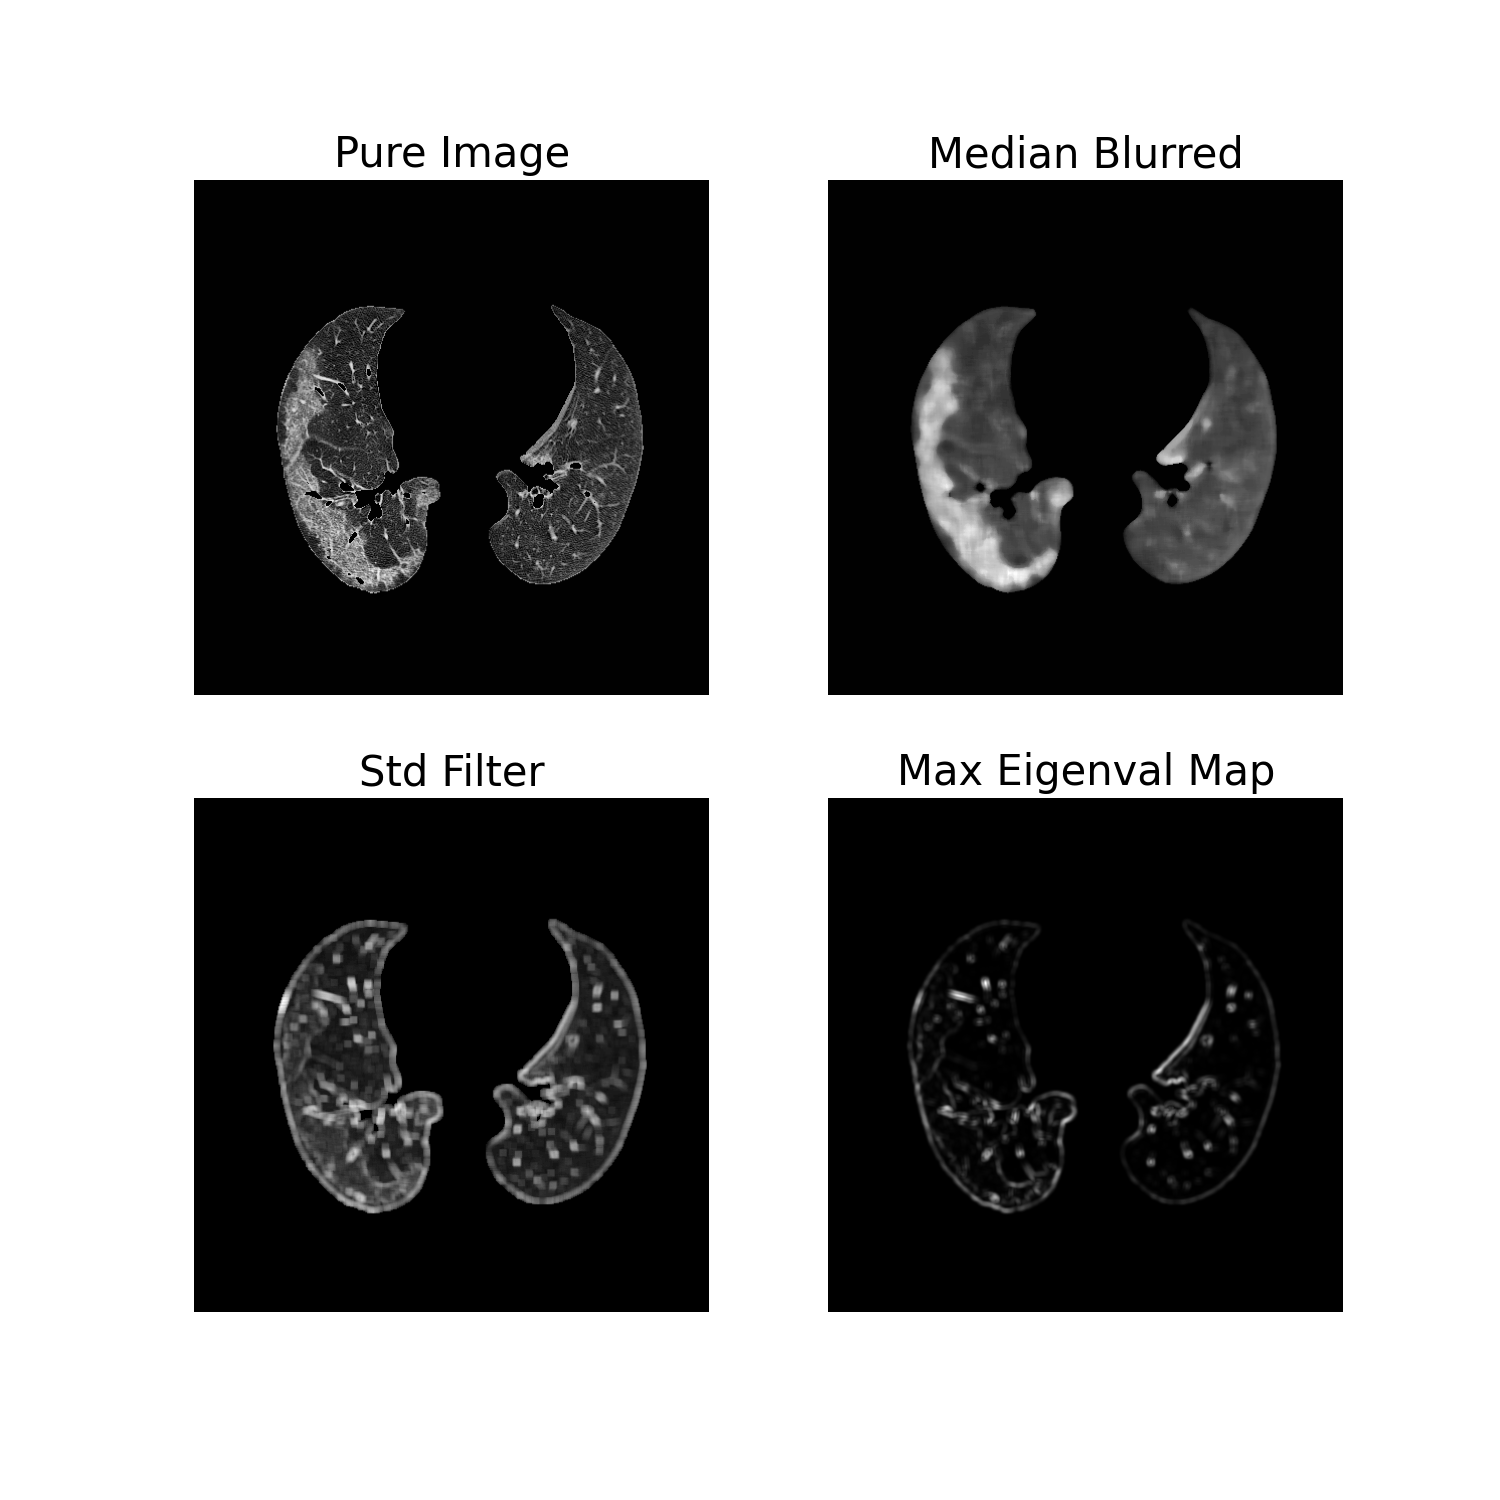
\includegraphics[scale=.55]{Multi_Channel.png}
			\caption{Channels of the image. From left to right and from top to bottom the image after the histogram equalization, the gamma correction, the median blurring and the std filtering. These channels allow us to consider information about single voxel, neighbouring voxels and their variability. The histogram equalization is applied over small $10\times 10$ areas to avoid over-amplification of the contrast. The gamma correction was performed using $\gamma = 1.5$, and the median and std filter kernel sizes are respectively $11$ and $3$. Each image is normalized according to the mean and standard deviation of the whole scan. }\label{fig:MultiChannel}
		\end{figure}
	
	In \figurename\,\ref{fig:MultiChannel} I have displayed the four different channels of the image. Each channel allows us to consider different information.

	The histogram equalized and the gamma-corrected images allow to take into account information about the single voxel. The histogram equalization is applied to enhance the image contrast by improving GL usage. For each slice, the histogram is equalized considering only a $10\times 10$ area, to take care of the over-amplification of the contrast.

	The gamma correction is a non-linear operation and is used to decode the luminance and to make in evidence the low contrast regions. 

	The median blurring allows us to consider also the information about the neighbourhood voxels, allowing the reduction of the outliers. The usage of the filter is justified since the lesions involve several closest voxels.

	The last channel consists of the image after the application of a local standard deviation filter. This filter consists of the replacement of each pixel value with the standard deviation of its neighbourhood. It helps us to distinguish the bronchial structures and motion artefacts not removed during the lung segmentation. 

	Each channel of the image is normalized according to means and standard deviation of the whole scan; because of the k-means clustering.

\end{document}